\documentclass[a4paper]{article}
% Eso define el tipo de documento.
% `article` se divide en secciones y tiene el resumen pegado al texto
\usepackage{graphicx}
% Son como los import de librerias. `graphicx` es para importar imagenes
\usepackage{listings}
% `listings` es para insertar los codigo fuente
\usepackage[utf8]{inputenc}
% `utf8` es para no tener problemas con el encoding (acentos, etc.)
\usepackage{caption}
% Para cambiar leyenda de figuras

\title{Trabajo Práctico Nro. 3:\\``Sistema de llenado\\y vaciado de un tanque''}
\author{Amodey, Leandro - leandroamodey@gmail.com
\and Monti, Matías - matiasmonti@hotmail.com
\and Quinteros, Fernando - lordfers@gmail.com
\and Araneda, Alejandro – eloscurodeefeso@hotmail.com}
\date{1er. Cuatrimestre 2020\\Jueves, 25 de Junio}
% `title`, `author` y `date` es informacion que todos los archivos tienen.

\def\teacher{Ing. Jorge H. Doorn
\and Ing. Matías Presso}
% Variable propia para definir profesores.

\captionsetup{justification=centering,labelsep=period,font={small},%
labelfont=bf,textfont=it}
% Las leyendas deben ser chicas y en italica, separadas con punto
% y la numeración en negritas, todo centrado.
\renewcommand{\figurename}{Figura}
% Con eso cambiamos como salen los titulos de las figuras.
\renewcommand{\abstractname}{Resumen}
% Con eso le cambio en titulo del resumen
\renewcommand{\refname}{Referencias}
% Cambia el titulo de la bibliografia
\let\originalcite\cite
\renewcommand{\cite}[2][]{\textsuperscript{\originalcite{#2}}}
% Cambiamos el estilo de las citas bibliograficas
\makeatletter\let\@afterindentfalse\@afterindenttrue\makeatother
% Cambiamos \@afterindentfalse por \@afterindenttrue para indentar primer parrafo
\let\originalappendix\appendix
\renewcommand{\appendix}{%
    \newpage\originalappendix\pagenumbering{gobble}%
    % Empezar apéndices en nueva pagina sin numeracion
    \renewcommand\thesection{Anexo \Alph{section}}
    % `thesection` es como se numeran los apendices
    \setcounter{secnumdepth}{1}
    % Contarlas secciones de apendice
}
\setcounter{secnumdepth}{0}
% No se numeran las secciones pero si estan en el TOC 
\newenvironment{ejercicios}
    {\setcounter{secnumdepth}{3}
    \renewcommand\thesubsection{Ejercicio \arabic{subsection}}}
    {\setcounter{secnumdepth}{0}}
% Defino un enviroment para numerar ejercicios

\begin{document}
% Arranca el documento

% Pagina propia de titulo
\begin{titlepage}\renewcommand\and\par\centering\makeatletter
    
\includegraphics{logo.png}\par
    {\Large Ingeniería en Computación \par}\vspace{0.5cm}
    {\LARGE Laboratorio de Microprocesadores \par}\vfill
    {\huge \@title \par}\vfill
    Grupo 2:\par
    \@author\vfill
    Práctica entregada:\par
    \@date\vfill
    Docentes:\par
    \teacher\vspace{1cm}\makeatother
\end{titlepage}

\begin{abstract}

    En el presente trabajo realizaremos el análisis y diseño para la implementacion
    de un sistema que se ocupe del llenado y vaciado de un tanque mediante el uso de 
    microcontroladores y elementos eléctrìcos y electrónicos.
    Como entregable del presente trabajo se realizará el presente informe junto con los archivos 
    del esquemático del sistema, y una simulación del mismo funcionando.

\end{abstract}

\section{Introducción}


\section{Descripción de la Práctica}

\subsection{Enunciado}

A continuación transcribimos el enunciado original de la práctica.
Del mismo tomamos los puntos teóricos que son descriptos en la 
Introducción y fue la base para realizar el diseño detallado en la seccion correspondiente.

\begin{quotation}

    \begin{center}
        
        Taller de Microprocesadores Trabajo Practico  3                

    \end{center}
    \begin{abstract}
    Diseñar un sistema que permita llenar y vaciar un tanque de líquido con dos bombas independientes. 

    El inicio de llenado del tanque debe realizarlo mediante un botón (o señal digital externa ) y deben ingresar 500 lts (o cierto volumen fijo). El vaciado también puede realizarse con un botón o señal digital externa. El llenado no puede realizarse si el tanque esta por encima de cierto nivel, y el vaciado deber finalizar con un nivel mínimo en el tanque para proteger que la bomba no funcione sin líquido. El vaciado no puede en caso que no existe ese nivel mínimo y debe indicarse con una luz que el tanque se encuentra en su mínimo nivel.
    \end{abstract}
\end{quotation}

\subsection{Plataforma de Desarrollo}

Utilizamos el lenguaje C para programar las aplicaciones. Presentamos
una copia de los mismos como anexos.

Para nuestro desarrollo utilizamos el compilador MPLAB 
XC8\cite{bib:compilador} de la empresa Microchips. El mismo es el 
diseñado específicamente para la línea de microcontroladores de 8 bits
a la que pertenece el PIC12F675.

El diseño y simulación del esquemático correspondiente a cada 
aplicación se realiza con el software Proteus\cite{bib:simulador} de 
la compañía Labcenter Electronics.

\subsection{Instrucciones de Compilación y Ejecución}

Para la compilación del firmware utilizamos la línea de comandos en 
una terminal. Como parámetro a la ejecución del compilador agregamos
el modelo del microcontrolador donde se instala el software. Éste es 
el método recomendado por el desarrollador por sobre el de incluir en 
el código mismo los archivos de encabezado para el preprocesador con 
las configuraciones específicas del modelo. Por ejemplo, para el 
primer ejercicio utilizamos:

\begin{center}\ttfamily 
	xc8 --chip=12f675 ejercicio1.c
\end{center}

El compilador genera un archivo {\ttfamily .hex} que es el que
agregamos a las propieda-des del microcontrolador solicitadas 
por el software Proteus para la simulación del circuito. Allí también 
indicamos tanto la frecuencia del reloj y la palabra que representa 
los bits de configuración que debieran ser impresos en la memoria del
integrado junto con el código ejecutable. 

\section{Diseño del sistema}

    \subsection{Caso de uso}

    Completar

    \subsection{Diagrama de arquitectura}

    Completar

    % --- Para insertar una imagen escriban de acá
    \begin{figure}[h]\centering
    % La opcion `[h]` es para "here", pero puede cagarse en eso.
    % No usar "la imagen que sigue" sino la referencia.
        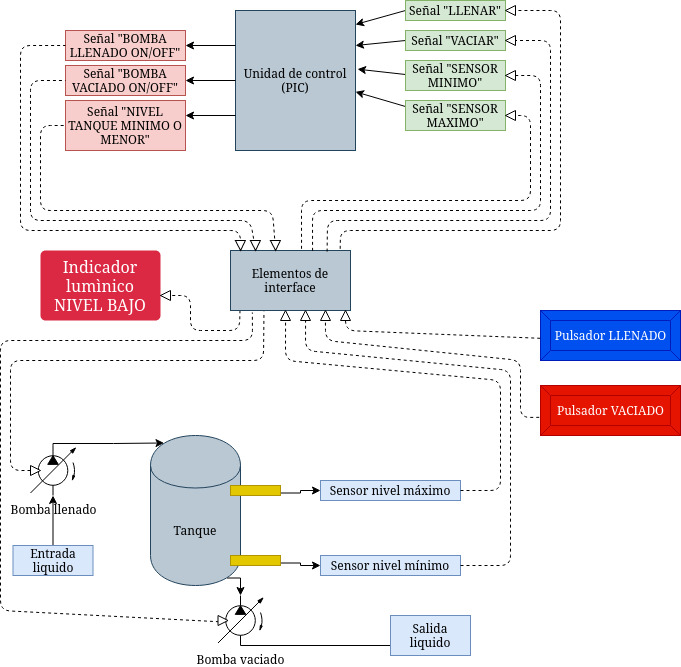
\includegraphics[height=12cm]{diagrama_sistema.jpg}
        \caption{Esquema del sistema general.}\label{fig:esquematico1}
    \end{figure}
    % --- hasta acá.

    \subsection{Esquemático del circuito.}

    \subsection{Descripción de funcionamiento.}



    
\section{Análisis y simulación.}

\subsection{Completar las subsecciones}

\section{Conclusiones}

Completar

\noindent\rule{\textwidth}{1pt}
% Linea horizontal sin identacion y del ancho del texto

\begin{thebibliography}{9}
% Comienza la bibliografia
% El "9" indica que el espacio para imprimir "9" es de la mayor referencia

% Para agregar una entrada a la bibliografia repetir de aca
\bibitem{bib:boylestad} 
Boylestad, R. \& Nashelsky, L. (2002). 
\textit{``Electronic devices and circuit theory"}.
Upper Saddle River, N.J: Prentice Hall.
% Hasta aca termina la referencia

\bibitem{bib:compilador}
\textit{``Microchip MPLAB XC8 C Compiler"}
(Versión 2.10; Microchip Technology Inc.: 2019).
Recuperado de https://www.microchip.com/mplab/compilers

\bibitem{bib:simulador}
\textit{``Proteus 8 Professional"} 
(Versión 8.5 Service Pack 0; Labcenter Electronics: 2016).
Recuperado de https://www.labcenter.com/

\bibitem{bid:datasheet}
Microchip (2010).
\textit{``PIC12F629/675 Data Sheet. 8-Pin FLASH-Based 8-Bit CMOS 
Microcontrollers''.}
EE.UU. Recuperado de 
http://ww1.microchip.com/downloads/en/DeviceDoc/41190G.pdf

\bibitem{bid:Transistor}
``¿Qué es un transistor y como funciona?'' (2020).
Recuperado de 
https://www.ingmecafenix.com/electronica/el-transistor/

\end{thebibliography}


\appendix

\section{}\label{ane:monitoreo}
A continuación listamos en extenso el código fuente en lenguaje C
correspondiente al \ref{ej:monitoreo}. La descripción de su 
funcionamiento puede encontrarse en la sección de Diseño y 
Simulación.

%\lstinputlisting[language=C,basicstyle=\ttfamily\scriptsize,numbers=left]{../ejercicio1.c}
% `lstinputlisting` inserta el codigo.
% Lo configuro para C, en monospace y tamaño chico, con numeracion a la izquierda.
% Recordar que el archivo tiene una direccion relativa a esta carpeta.
% Los de verdad van a estar en la carpeta padre "../ejercicio1.c"

\newpage
% Incluir salto de pagina de manera manual en cada apendice.
\section{}\label{ane:Corriente alterna o considerable}
A continuación podran ver el  código fuente en lenguaje C correspondiente
al \ref{ej:Resistor}. La descripción de su funcionamiento puede encontrarse en
la sección de Diseño y Simulación.

%\lstinputlisting[language=C,basicstyle=\ttfamily\scriptsize,numbers=left]{../ejercicio2.c}

\end{document}
